\section{Результаты}
\subsection{Максимум распознающего функционала}
\begin{figure}[H]
\centering
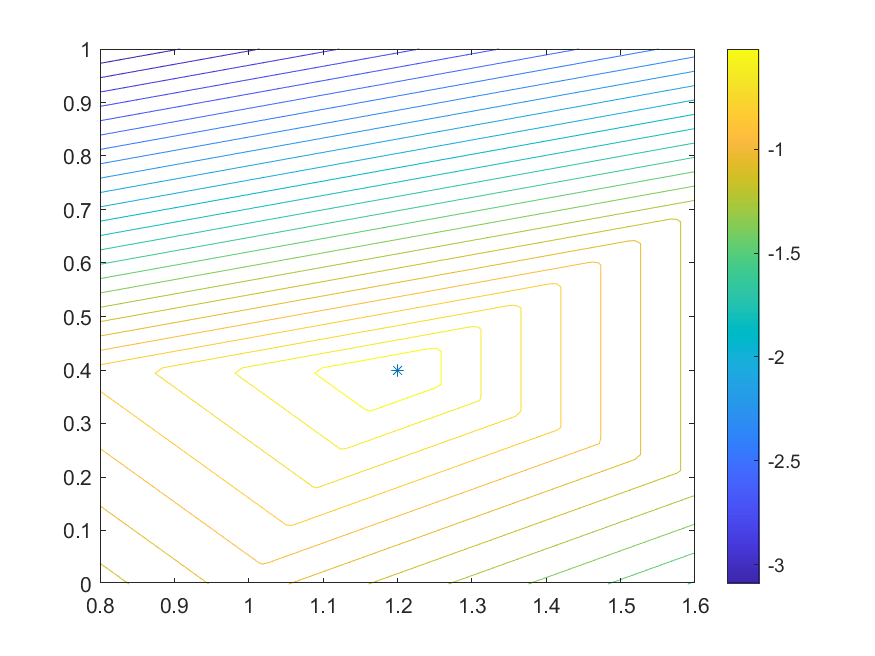
\includegraphics[width=0.75\textwidth]{Graphics/maxTol.png}
\caption{Расположение максимума распознающего функционала} 
\end{figure}
Максимум со значением $T=-0.4$ расположен в точке $\tau=(1.2,0.4)$.
\subsection{Достижение разрешимости за счёт коррекции правой части}
Положим вектор весов $v$ равным единичному вектору, а $K=1.2\cdot |T|$.
\begin{figure}[H]
\centering
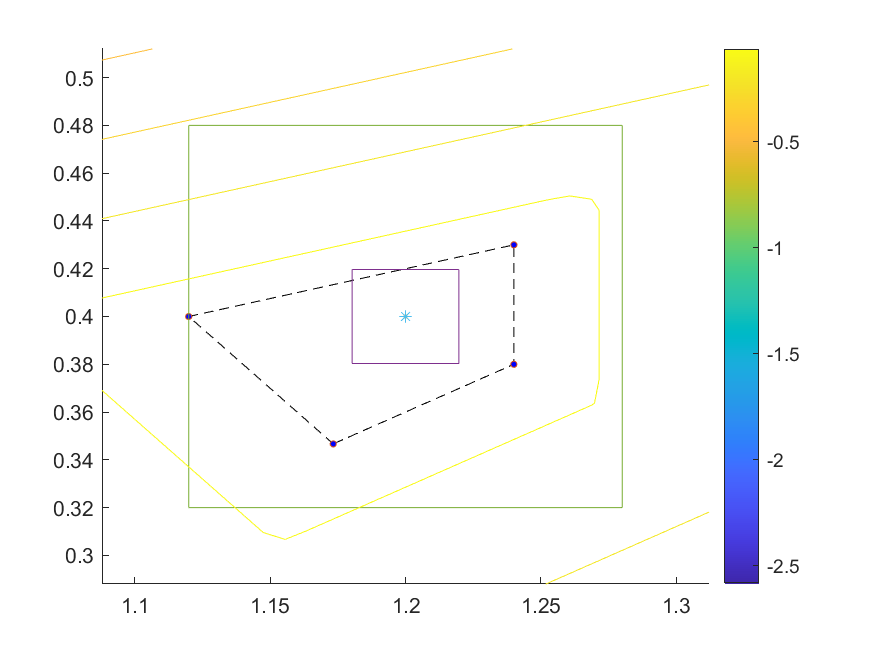
\includegraphics[width=0.75\textwidth]{Graphics/biasCorr.png}
\caption{Допусковое множество решений с скоректированной правой частью} 
\end{figure}
\noindent На данном рисунке фиолетовый квадрат имеет сторону $2\cdot \mathrm{ive}$, а зелёный - $2\cdot \mathrm{rve}$
\subsection{Достижение разрешимости за счёт коррекции матрицы}
Положим 
\begin{equation}
    \mathbf{E}=
    \begin{pmatrix}
[-0.3, 0.3]  &  [-0.3, 0.3] \\
0  &  [-1, 1] \\
[-0.7, 0.7]  &  0
\end{pmatrix}
\end{equation}
\begin{figure}[H] \label{MatrixCorrSet}
\centering
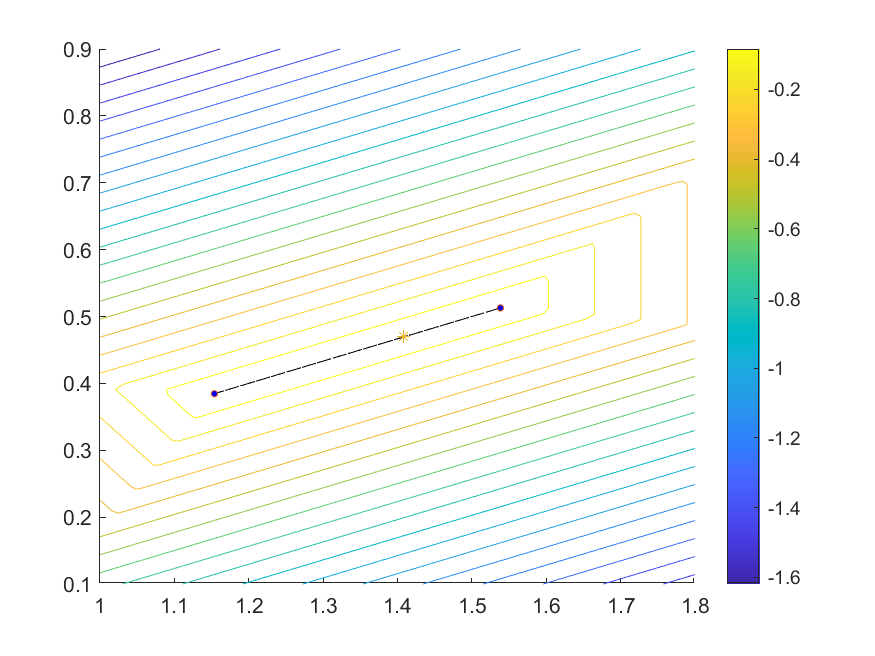
\includegraphics[width=\textwidth]{Graphics/matrixCorr.png}
\caption{Допусковое множество решений с скоректированной матрицей} 
\end{figure}
\subsection{Управление положением argmax}
\subsubsection{Путём корректировки матрицы в целом}
Представим матрицу сужения как
\begin{equation}
    \mathbf{E}=
    \begin{pmatrix}
[-e, e]  &  [-e, e] \\
0  &  [-1, 1] \\
[-2 * e, 2 * e]  &  0
\end{pmatrix}
\end{equation}
и будем менять $e$ в интервале $[0, 0.3]$ с шагом $0.05$.
\begin{figure}[H]
\centering
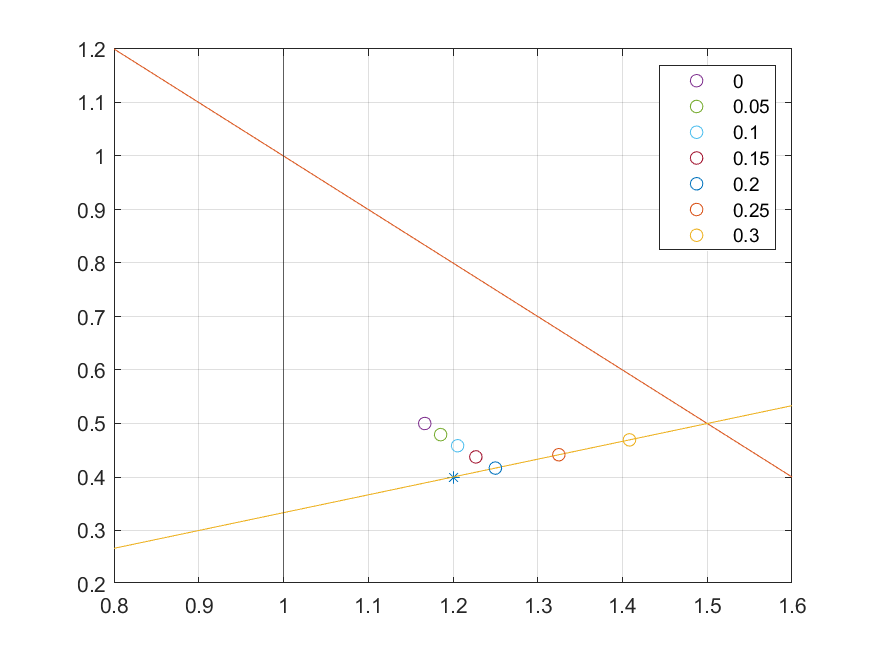
\includegraphics[width=0.8\textwidth]{Graphics/fullCorr.png}
\caption{Положение argmax при корректировке матрицы в целом} 
\end{figure}
\subsubsection{Путём корректировки первой строки}
Представим матрицу сужения как
\begin{equation}
    \mathbf{E}=
    \begin{pmatrix}
[-e, e]  &  [-e, e] \\
0  &  [-1, 1] \\
[-0.35, 0.35]  &  0
\end{pmatrix}
\end{equation}
и будем менять $e$ в интервале $[0, 0.35]$ с шагом $0.07$.
\begin{figure}[H]
\centering
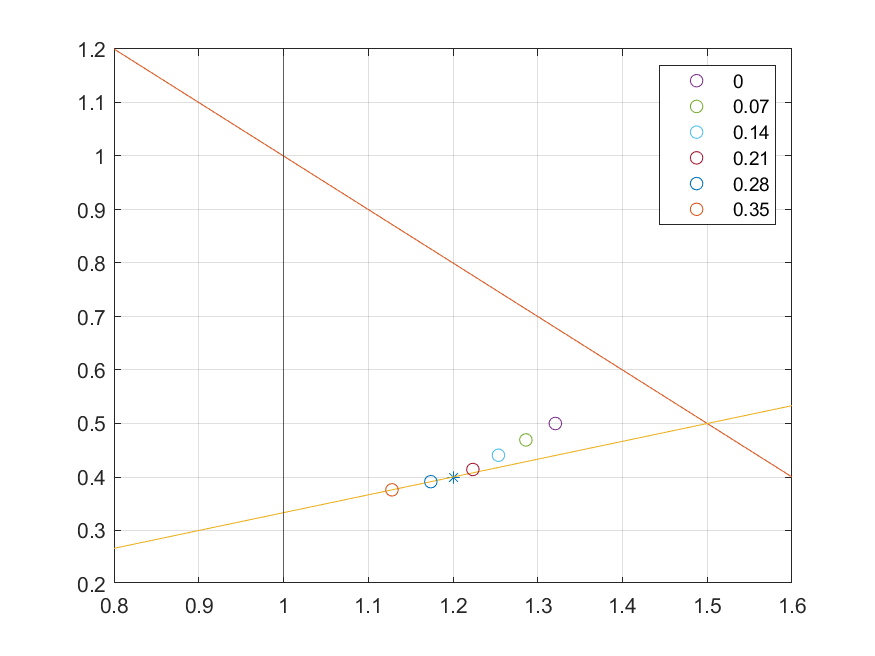
\includegraphics[width=0.8\textwidth]{Graphics/row1Corr.png}
\caption{Положение argmax при корректировке первой строки} 
\end{figure}
\subsubsection{Путём корректировки второй строки}
Представим матрицу сужения как
\begin{equation}
    \mathbf{E}=
    \begin{pmatrix}
[-0.25, 0.25]  &  [-0.25, 0.25] \\
0  &  [-e, e] \\
[-0.35, 0.35]  &  0
\end{pmatrix}
\end{equation}
и будем менять $e$ в интервале $[0, 1]$ с шагом $0.2$.
\begin{figure}[H]
\centering
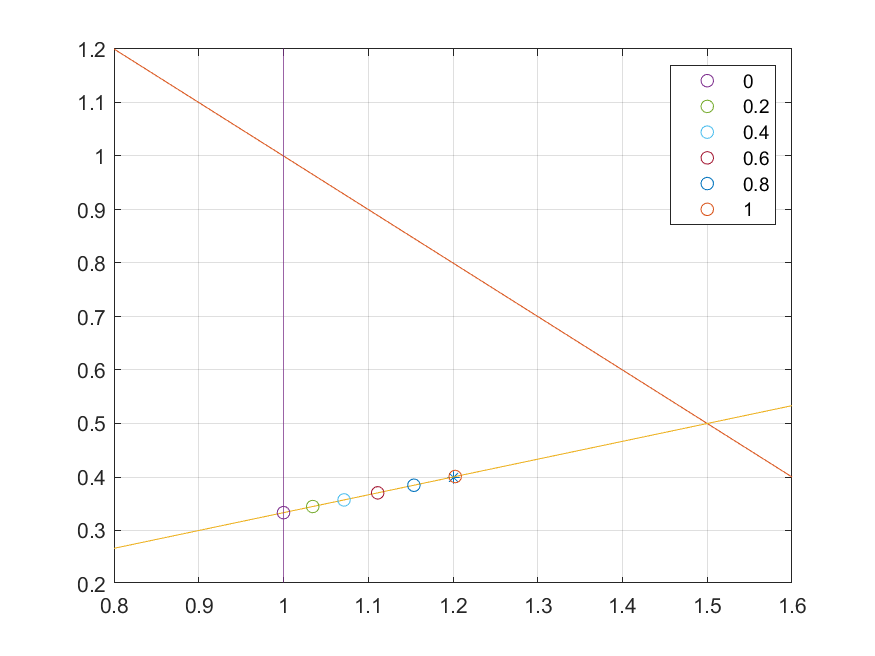
\includegraphics[width=\textwidth]{Graphics/row2Corr.png}
\caption{Положение argmax при корректировке второй строки} 
\end{figure}
\subsubsection{Путём корректировки третьей строки}
Представим матрицу сужения как
\begin{equation}
    \mathbf{E}=
    \begin{pmatrix}
[-0.25, 0.25]  &  [-0.25, 0.25] \\
0  &  [-1, 1] \\
[-e, e]  &  0
\end{pmatrix}
\end{equation}
и будем менять $e$ в интервале $[0, 0.6]$ с шагом $0.1$.
\begin{figure}[H]
\centering
\includegraphics[width=0.85\textwidth]{Graphics/row3Corr.png}
\caption{Положение argmax при корректировке третьей строки} 
\end{figure}